\documentclass{acmsiggraph}
\usepackage[english]{babel}
\usepackage[T1]{fontenc}
\usepackage[latin1]{inputenc}
\usepackage{float, enumitem, footnote, multirow}
\usepackage[font=scriptsize,labelfont=bf, justification=centering, format=hang]{caption}
\usepackage{subfig}
\usepackage{amsmath, amsthm, amssymb}
\usepackage[linesnumbered,ruled,vlined]{algorithm2e}
\usepackage{microtype}
\usepackage{lmodern}
\usepackage{listings}
\lstset{
	basicstyle=\footnotesize
}
\graphicspath{{../figures/}}

\newcommand\mycommfont[1]{\footnotesize\ttfamily{#1}}
\SetCommentSty{mycommfont}

\title{Advanced Learning for Text and Graph Data\\
Project report}

\author{Maha ELBAYAD\\
{\large (Kaggle team : ELBAYAD)}\\
\large{Ecole Normale Superieure de Cachan - Master MVA}\\
\\\texttt{maha.elbayad@student.ecp.fr}}
\pdfauthor{Maha ELBAYAD}

\DeclareMathOperator\disp{disp}
\DeclareMathOperator\Jacc{Jacc}
\DeclareMathOperator\sigmoid{sigmoid}
\DeclareMathOperator\diffin{diff_{in}}
\DeclareMathOperator\ind{in}
\DeclareMathOperator\Adar{Adar}
\newcommand{\G}{\mathbf{G}}
\newcommand{\Gac}{\mathbf{GAC}}
\newcommand{\Gaa}{\mathbf{GAA}}
\begin{document}
\maketitle

\section{Introduction}
This project aims at predicting missing links on a citation network where edges have been deleted at random. The citation network is set to be a graph where nodes are research papers and an edge $(u,v)$ exists if article $u$ has cited article $v$.

\section{Outline}
We distinguish three different phases, first the pre-processing and feature engineering where we design features based on meta-data provided on each article of the network as well as textual information extracted mainly from the articles' abstracts and topological information from the main citation network or other auxiliary graphs introduced below. The second phase is learning a classifier on these engineered features to predict whether an edge exists or not. We will compare different classifiers and features selection techniques to boost the classification performance evaluated by the F1-score.

\section{The datasets}
Our articles corpus consists of 27770 articles where we're provided with the paper title, its publishing year, its authors with their affiliations, the publishing journal and the abstract/review of the article. We format the author name in the following format:

\begin{lstlisting}
Allen C. Hirshfeld (University of Dortmund)
author name : [`a.c.hirshfeld']
affiliation : [`univ dortmund']
\end{lstlisting}

The training set is of 615512 pairs of articles of which $x$ are citations link.
The articles in our corpus are published between 1992 and 2003 (cf. figure \ref{year}) and are published in different journals although a considerable number of journals are missing in the nodes information due mainly to the errors in parsing the \texttt{arXiv} meta-data, some of which were manually corrected (cf. figure \ref{jrn})
\begin{figure}[H]
\centering
\subfloat[Temporal diff\label{tempdiff}]{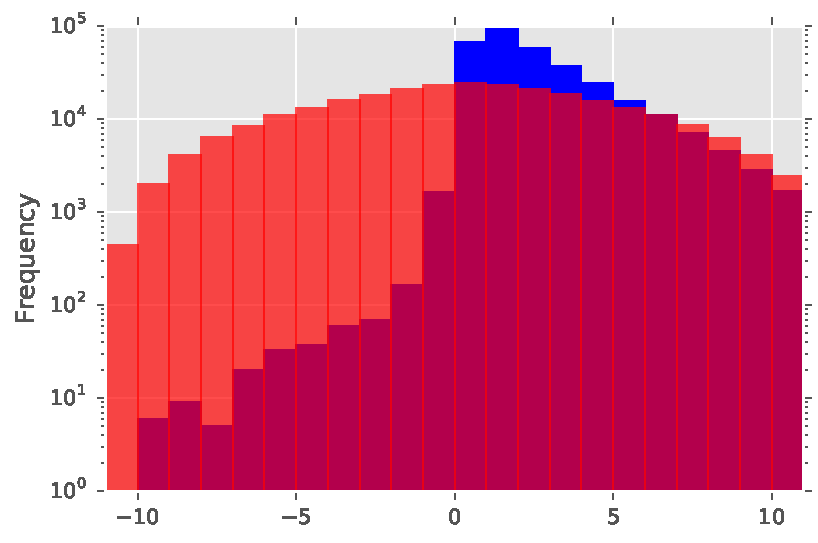
\includegraphics[height=2.7cm]{temporal_diff}}
\subfloat[Articles publication year\label{year}]{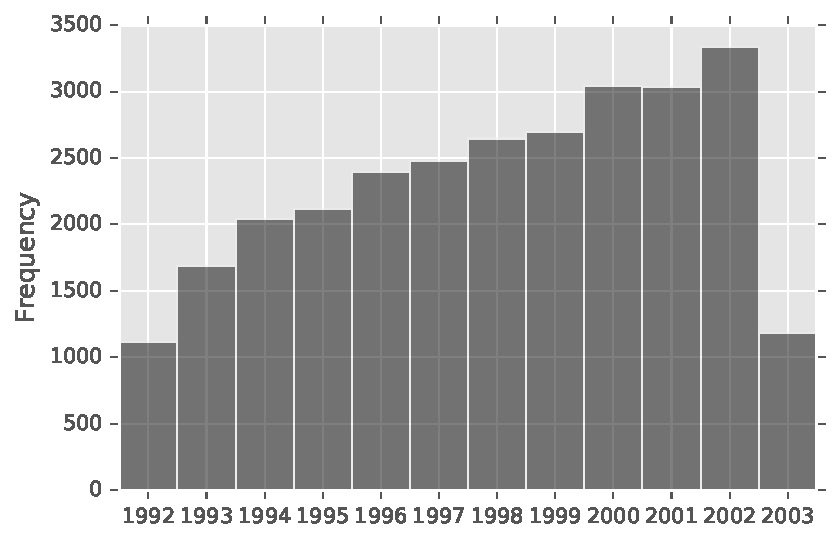
\includegraphics[height=2.7cm]{articles_years}}
\caption{Articles publication years and the temporal difference between the citing and cited articles (cf. attribute features)}
\end{figure}
\begin{figure}[H]
\centering
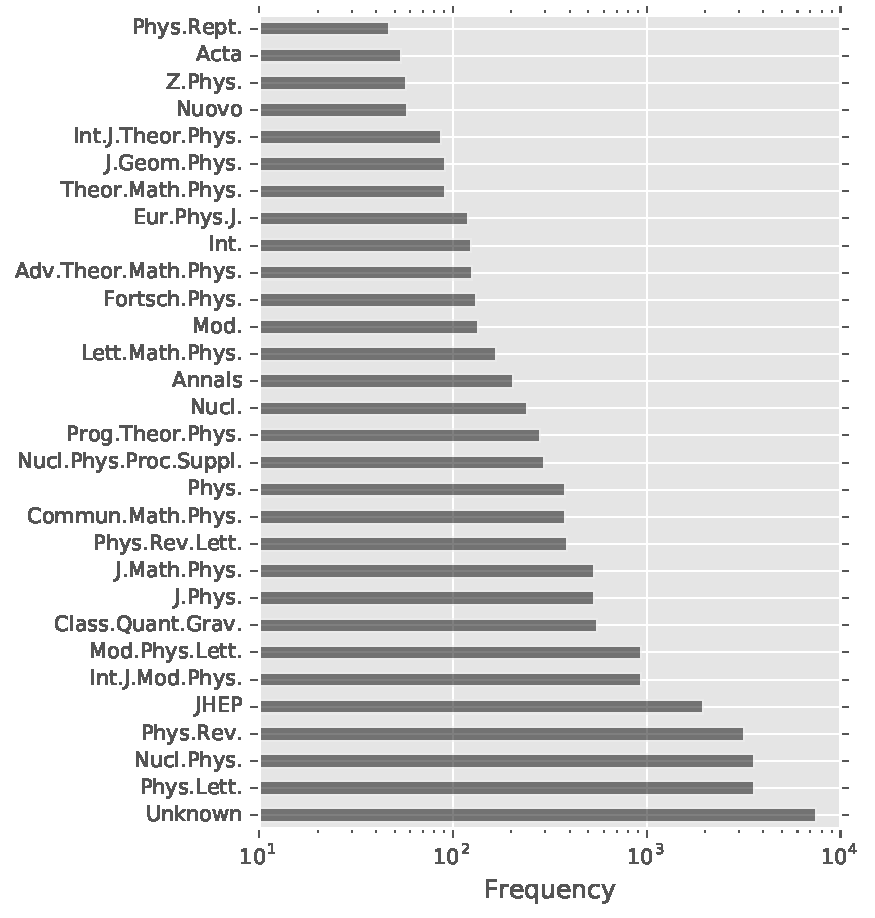
\includegraphics[width=7cm]{articles_journals}
\caption{Top 30 publishing journals in the corpus\label{jrn}}
\end{figure}
\section{Features engineering}
We consider the features chosen in Shibata et.al [2012], there are mainly three different groups of features: 
\subsection{Attribute features:}
Extracted from the nodes information
\begin{itemize}
\item \texttt{(title overlap)}  the titles overlap as the number of common words between the titles of the citing and cited papers.
\item \texttt{(temporal diff)} the difference in publication years. In fact researchers tend to cite recent papers with state of the art techniques to make relevant contributions (cf. figure \ref{tempdiff}). Although our graph is supposed to have edges from the citing to the cited articles which contradicts the fact that we have negative temporal difference, flipping those edges lowers the model performance.
\item \texttt{(self citation)} is it a self citation i.e. is there a common author between the two articles. It's likely for an author to mention her/his previous work to show the continuity of the research.
\item \texttt{(same journal)} are both articles published in the same journal.
\item \texttt{(common authors)} the number of the articles' common authors.
\item \texttt{(same affiliation)} Do authors have the same affiliation. To accurately compare the affiliations we map them to a features space via the \texttt{tf-idf} vectorizer or the \texttt{word2vec} deep learning model (cf. semantic features).
\end{itemize}

\subsection{Topolgical features:}
The main graph on which we predict the missing links is $\G$ whose nodes are the articles with edges from the citing to the cited article. We also considered two other graphs $\Gaa$ with the authors as nodes ans links between co-authoring authors and $\Gac$ with edges from the citing authors to the cited ones.
\begin{itemize}
\item \texttt{(common neighbors)} the number of common neighbors between the two articles $u$ and $v$ in undirected $\G$ i.e $|\Gamma_u\cap\Gamma_v|=|\Gamma_{uv}|$.
\item \texttt{(dispersion)} the dispersion between the two nodes in $\G$ that characterizes the edge's strength defined as:
\[\disp(u,v)=\sum_{s,t\in \Gamma_{uv}}d(s,t)\]
where $\Gamma_{uv}$ is the set of common neighbors between nodes $u$ and $v$ and $d(s,t)$ is the distance between the two nodes.
\item \texttt{(Jaccard coefficient)} the Jaccard coefficient defined in the undirected graph version of $\G$ as:
\[\Jacc(u,v)=\frac{|\Gamma_u\cap\Gamma_v|}{|\Gamma_u\cup\Gamma_v|}\]
\item \texttt{(Adar)} the Adamic/Adar ceffcient defined as:
\[\Adar(u,v) = \sum_{z\in\Gamma_{uv}} \frac{1}{\log|\Gamma_z|}\]
where having low-degree neighbors in common indicates a stronger connectivity. This feature is implemented for both the $\G$ graph and the $\Gaa$ graph. 
\item \texttt{(diff inlinks)} difference of in-degrees between the citing article $u$ and the cited article $v$:
\[\diffin(u,v) = \ind(v)-\ind(u)\]
where $\ind$ is the in-degree of a node in $\G$.
\item \texttt{(to cited)} number of the articles that cited the cited article $v$ i.e $\ind(v)$.
\item \texttt{(cited authority)} the cited authors ranks on $\Gac$ defined as the maximum Pagerank of the cited authors. These two last features reflect the fact that famous/successful articles are more likely to be cited and get more successful.
\item  \texttt{(authors same co)} if either one of the citing and cited authors are in the same community in undirected $\Gac$. For the logical reason that a community of researchers in the graph share the same interest in a specific topic.
\item \texttt{(articles same co)} if the citing and cited articles are in the same community in undirected $\G$.
\end{itemize}

For the community detection we compute the partition of the graph nodes which maximizes the modularity using the dendrogram generated by the Louvain algorithm (\texttt{community networkx API})
\begin{figure}[H]
\centering
\subfloat[][$\Gac$ degress\\8784 authors]{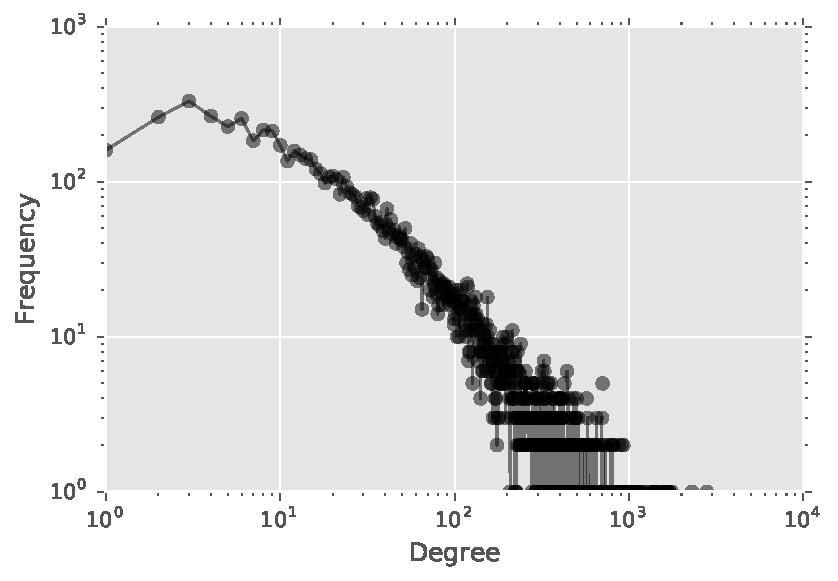
\includegraphics[width=4.3cm]{GAC_degrees}}
\subfloat[][$\Gac$ communities\\ 173 out of the 214 communities are singleton\\modularity = 0.73]{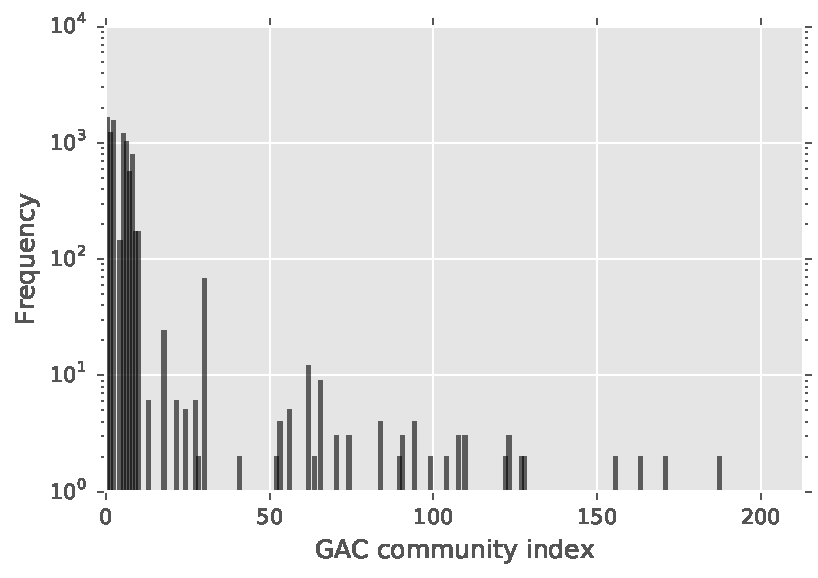
\includegraphics[width=4.3cm]{GAC_co}}\\
\subfloat[][$\G$ degress\\ 27770 articles]{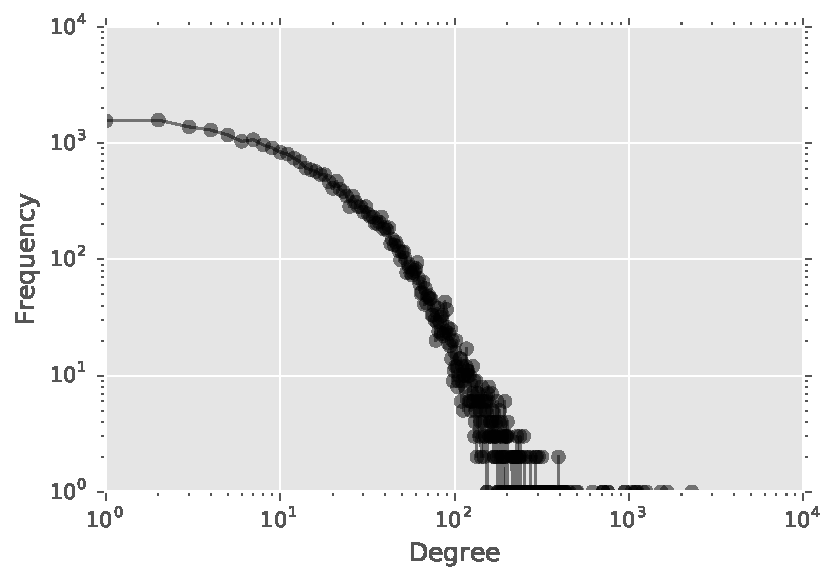
\includegraphics[width=4.3cm]{G_degrees}}
\subfloat[][$\G$ communities\\ 123 out of the 305 communities are singleton \\modularity = 0.97]{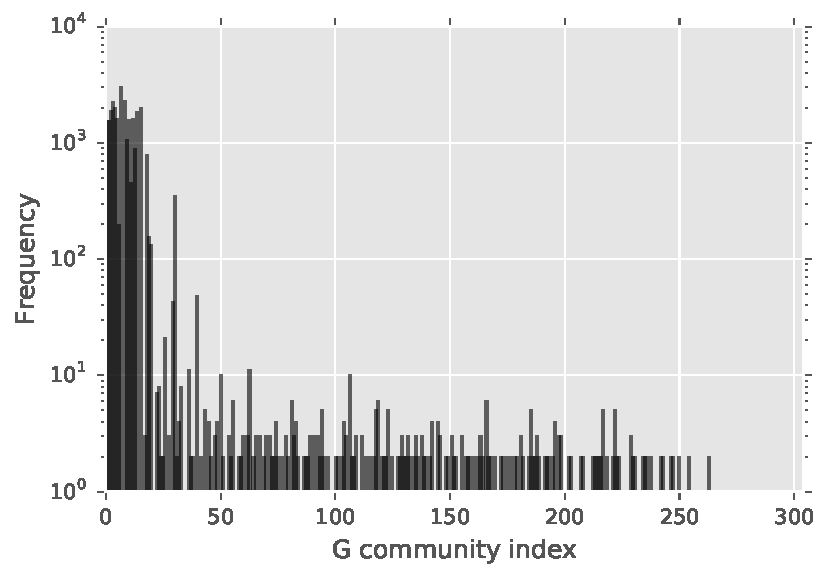
\includegraphics[width=4.3cm]{G_co}}
\caption{Communities detection in the citations graphs}
\end{figure}

\subsection{Semantic features:}
For the semantic features we focused mainly on the abstract, measuring the cosine similarities between vector representations of the abstracts. We experimented with both a \texttt{Tf-Idf} vectorization and a word embedding via the \texttt{word2vec} model.
\begin{table}[H]
\centering
\resizebox{\columnwidth}{!}{%
\begin{tabular}{|r|p{6cm}|c|c|}
\hline
parameter & description & abstract & affiliation \\
\hline
\hline
window & The maximum distance between the current and predicted word within a sentence & 15 & 3\\
\hline
size & The dimensionality of the feature vectors & 200 & 100\\
\hline
min\_count & Minimum total frequency to consider a word & 20 & 4\\
\hline
sample & Threshold for configuring which higher-frequency words are randomly down-sampled & 1e-3 & 1e-3\\
\hline

\hline
\end{tabular}}
\caption{Word2vec models' parameters (Gensim)}
\end{table}

\section{Features visualization}
To assess the quality of each feature we visualize an approximation of its density on the two different classes (existing citation - nonexistent citation)
\begin{figure}[H]
\centering
\subfloat[abstract similarity (\texttt{tf-idf})]{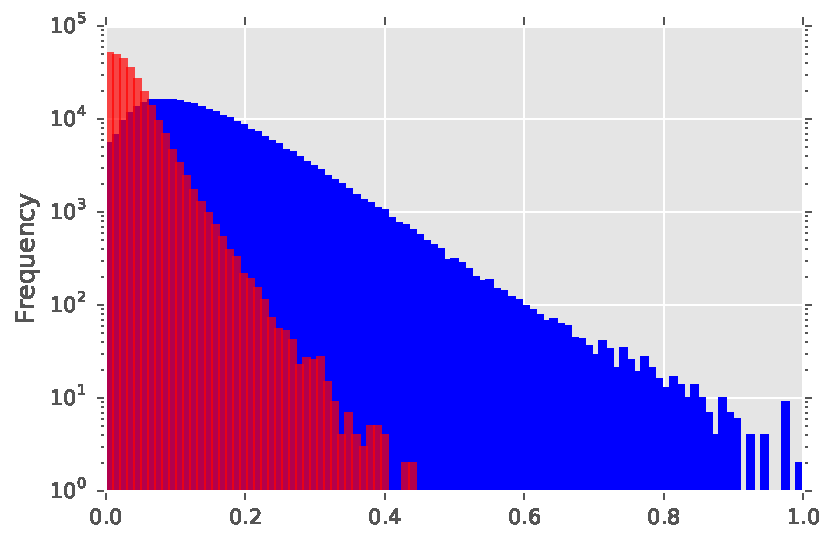
\includegraphics[width=4.3cm]{abstract_tfidf}}
\subfloat[abstract similarity (word2vec)]{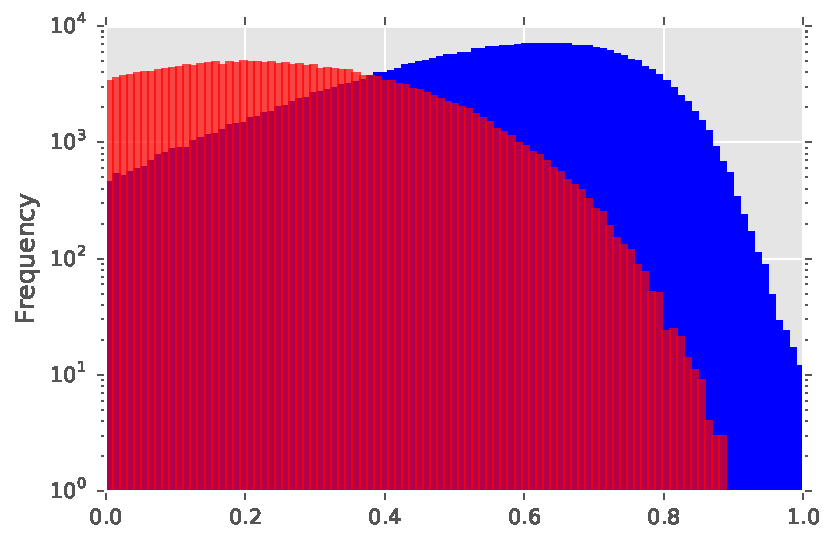
\includegraphics[width=4.3cm]{abstract_word2vec}}
\end{figure}
\begin{figure}[H]
\centering
\subfloat[affiliation similarity (\texttt{tf-idf})]{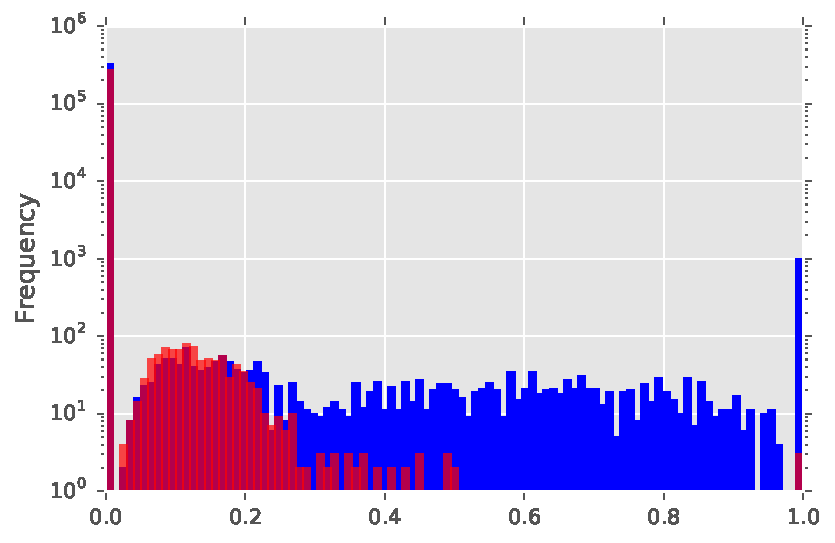
\includegraphics[width=4.3cm]{aff_tfidf}}
\subfloat[affiliation similarity (word2vec)]{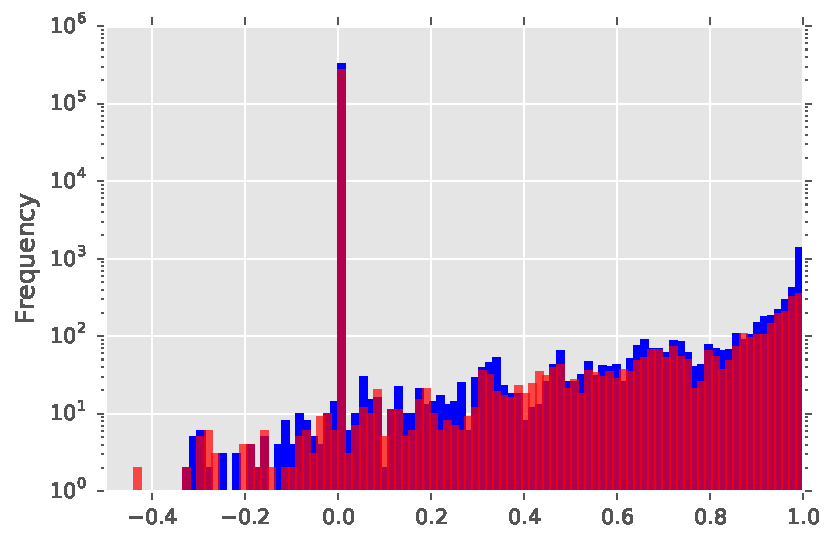
\includegraphics[width=4.3cm]{aff_word2vec}}
\end{figure}
\begin{figure}[H]
\centering
\subfloat[Jaccard coefficient]{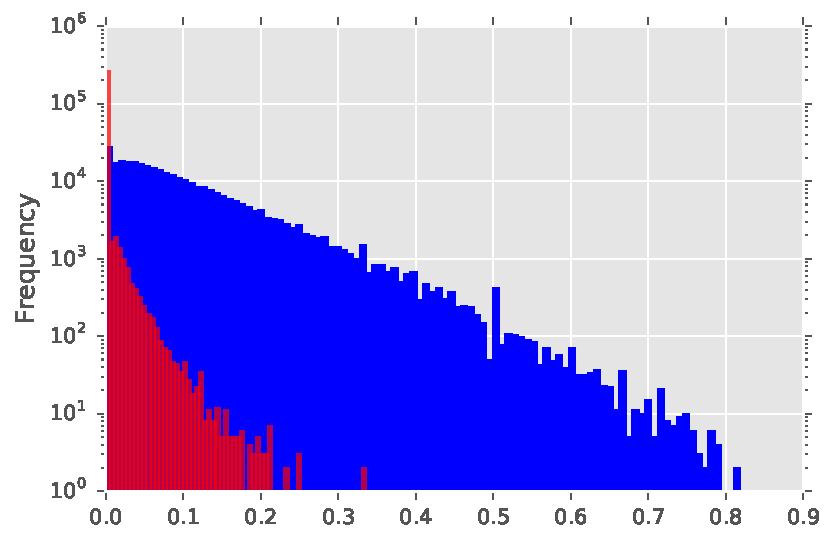
\includegraphics[width=4.3cm]{jaccard}}
\subfloat[Adamic/Adar]{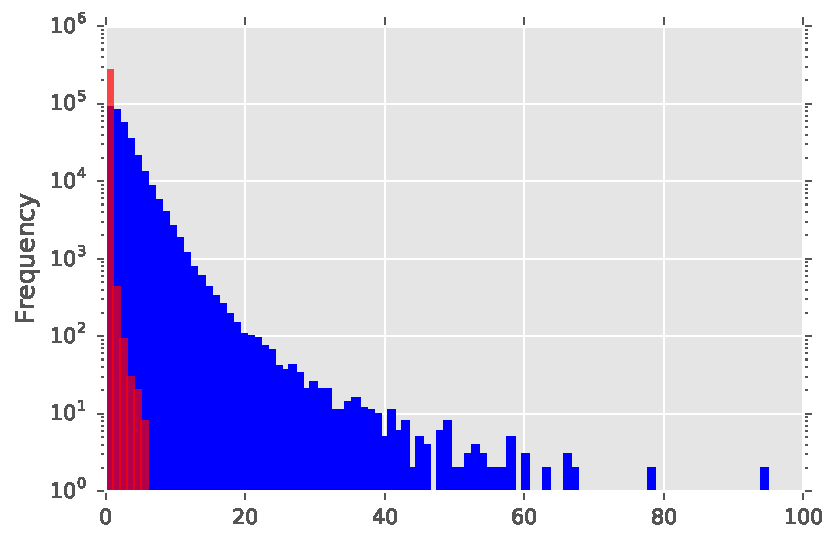
\includegraphics[width=4.3cm]{adar}}
\end{figure}
\begin{figure}[H]
\centering
\subfloat[To cited]{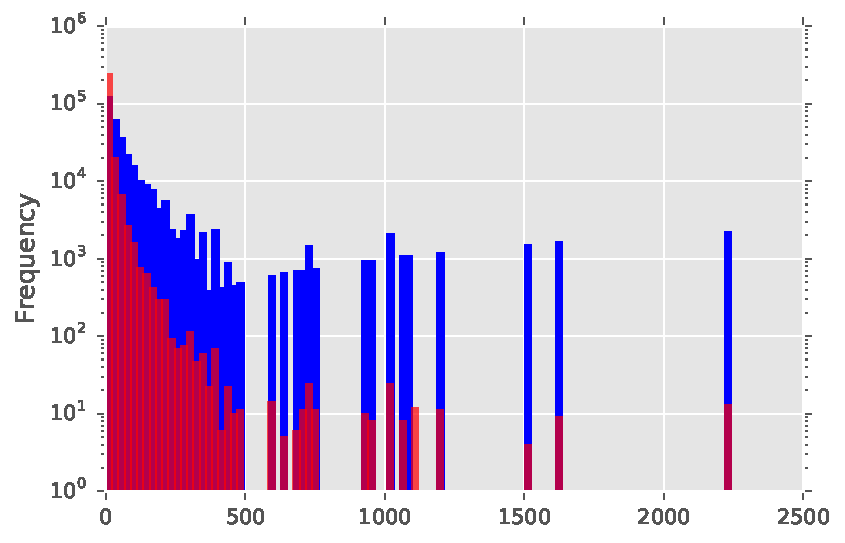
\includegraphics[width=4.3cm]{to_cited}}
\subfloat[Cited authority]{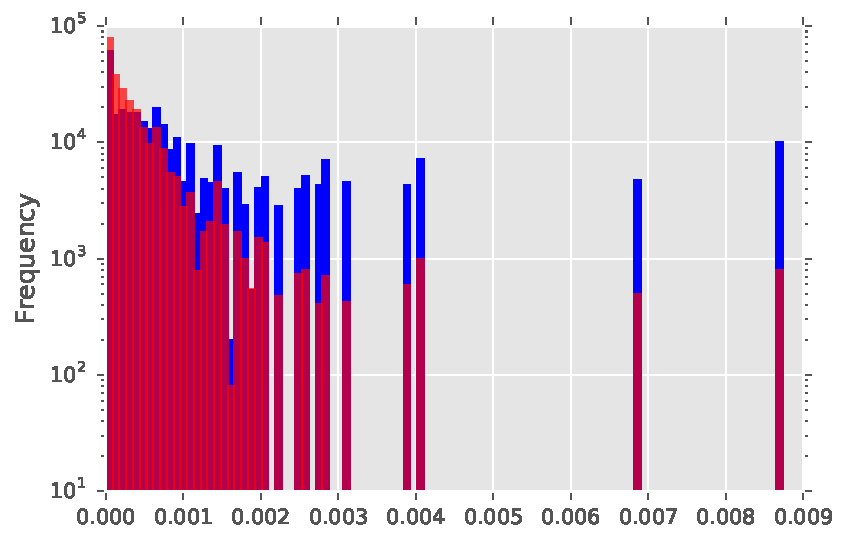
\includegraphics[width=4.3cm]{cited_authority}}
\end{figure}
\begin{figure}[H]
\centering
\subfloat[Dispersion]{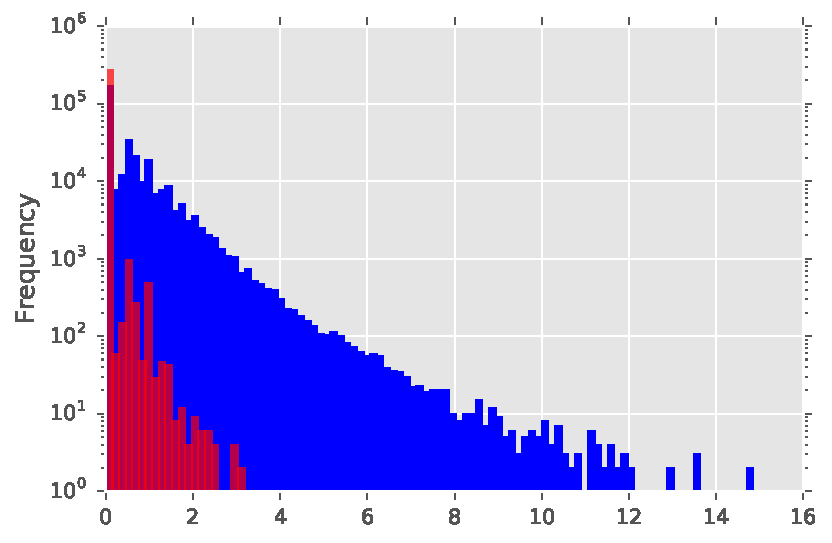
\includegraphics[width=4.3cm]{dispersion}}
\subfloat[diff inlinks]{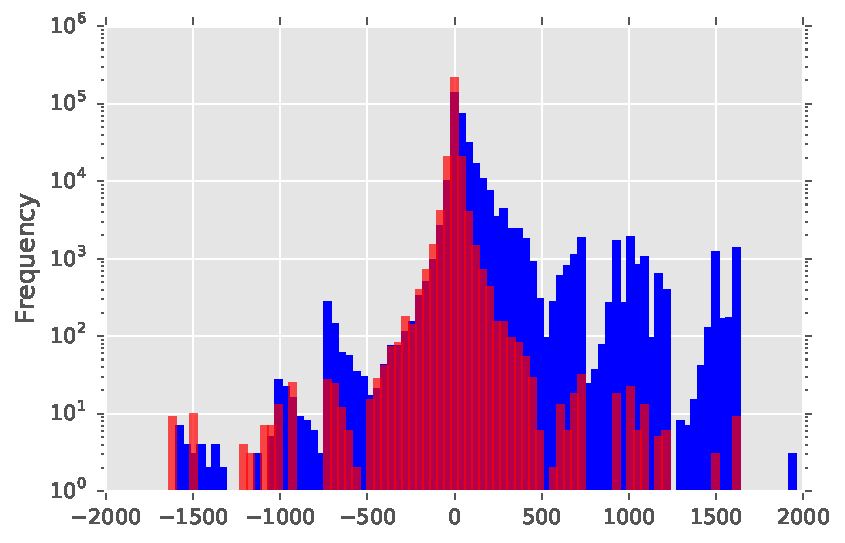
\includegraphics[width=4.3cm]{diff_inlinks}}
\end{figure}
\begin{figure}[H]
\centering
\subfloat[Common authors]{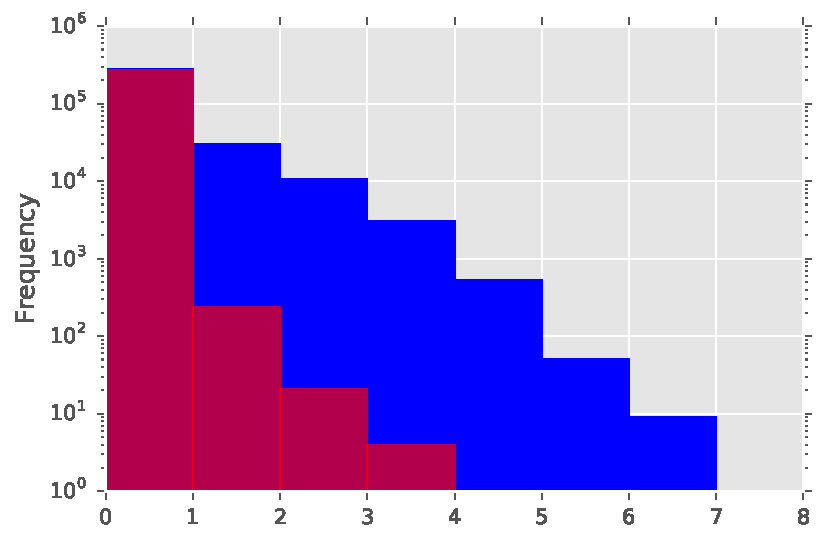
\includegraphics[width=4.3cm]{common_authors}}
\subfloat[Common neighbors]{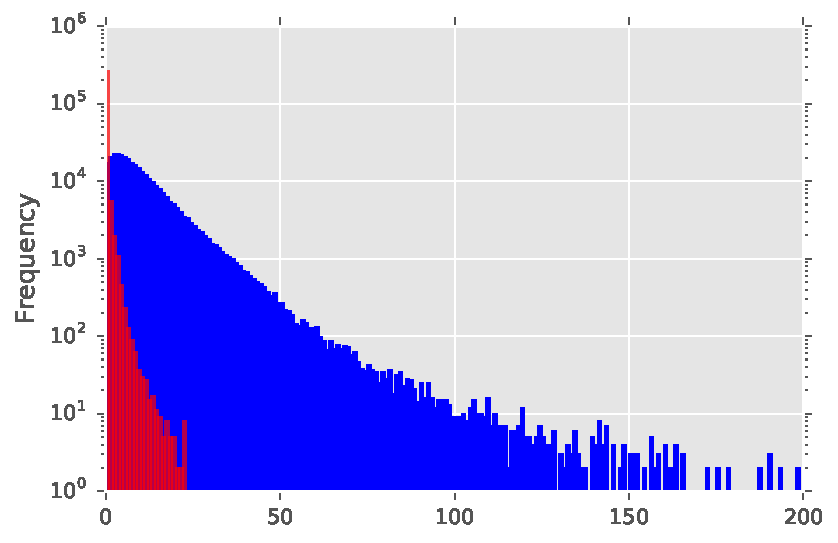
\includegraphics[width=4.3cm]{common_neighbors}}
\end{figure}
\begin{figure}[H]
\centering
\subfloat[Boolean features]{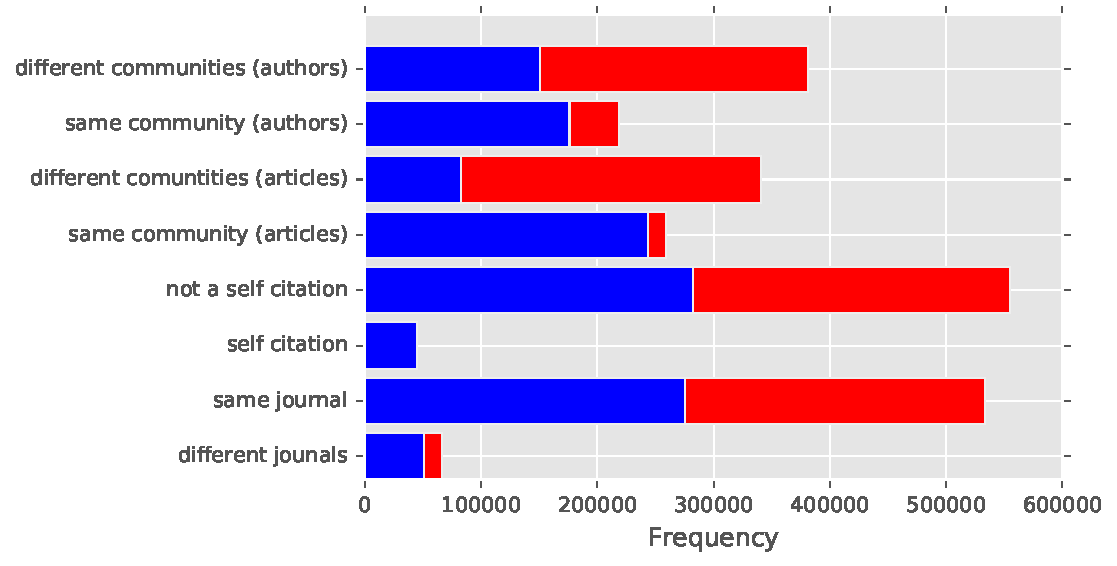
\includegraphics[width=6cm]{categorical}}
\caption{Features distribution in both classes. In red the negative class and in blue the positive class statistics}
\end{figure}

We note that refined coefficients such as the Jaccard, Adamic/Adar and Dispersion allow us to separate the two classes compared to simply counting the nodes difference of in-edges where the two classes heavily overlap. The cited authors authority evaluated by the Pagerank algorithms yields equivalent results to simply counting the times the target article was cited.
% \begin{figure}[H]
% \centering
% \subfloat[Degrees distribution ($\G$)]{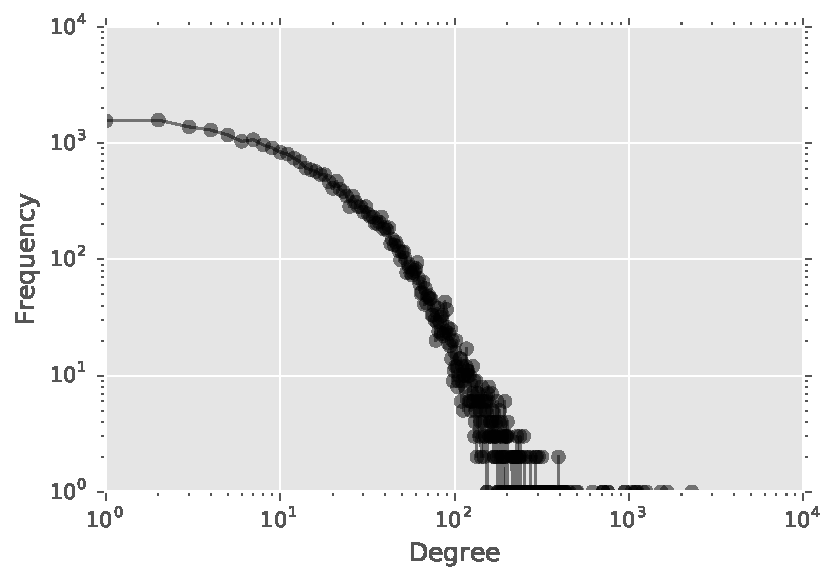
\includegraphics[width=4.3cm]{G_degrees}}
% \subfloat[Degrees distribution ($\Gac$)]{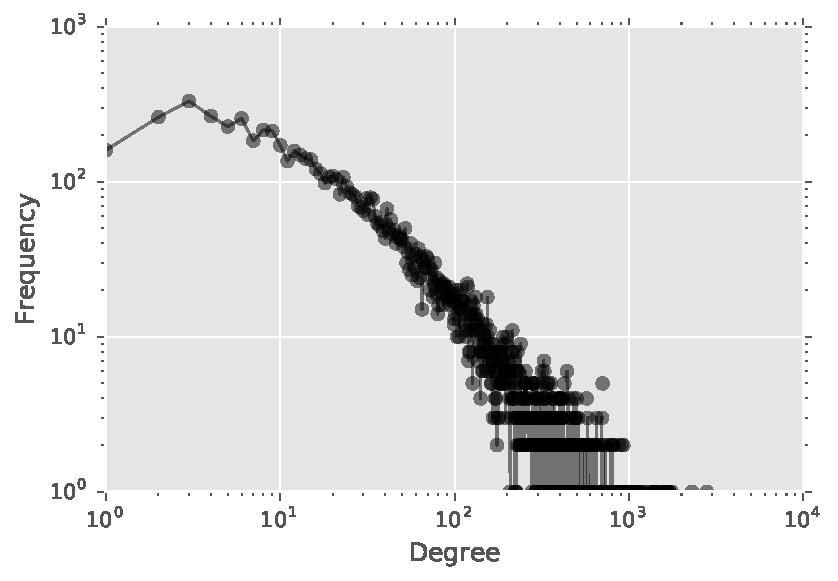
\includegraphics[width=4.3cm]{GAC_degrees}}
% \caption{}
% \end{figure}
\section{Classification and Model Selection}
For this project we experimented with different machine learning algorithms namely the C-SVM, Neural networks and random forests as well as logistic regression. To tune the model parameters for the SVM, RandomForest and Logistic Regression (from the Scikit learn library) we use the grid search to choose from a set of plausible parameters.

To select the most significant features we scale the design matrix (each feature would range between 0 and 1) and test the following techniques:
\begin{itemize}
\item \texttt{Recursive feature elimination:} we introduce all the above parameters to the model and then recursively remove the less significant features.
\item \texttt{Extremely Randomized Trees:} where random subsets of candidate features are tested
\item \texttt{Factor analysis:} to detect structure in the relationships between features.
\item \texttt{PCA:} To reduce the dimensionality of the problem.
\end{itemize}


\begin{figure}[H]
\centering
\subfloat[PCA first plane]{\includegraphics[width=4.3cm]{PCA}}
\subfloat[Factor Analysis first plane]{\includegraphics[width=4.3cm]{FA}}
\caption{Dimensionality reduction: Factor analysis yields better combined features adapted to the discrete features}
\end{figure}

\begin{table}[H]
\centering
\begin{tabular}{|c|c|c|}
\hline
Feature    &                rank(1)    &  importance (2)\\
\hline
\hline
dispersion               &    1    & 0.025259  \\
common neighbours        &    1    &  0.076234  \\
Jaccard coefficient      &    1	   &  \textbf{0.115636}  \\
Adar                     &    1   &  \textbf{0.082322}  \\
Adar authors             &    1   & 0.012043    \\
diff inlinks             &    1   &   0.024143  \\
to cited                 &    1   & 0.051572 \\
cited authority          &    5   &   0.026481   \\
articles same co         &    4   &    \textbf{0.284356} \\
authors same co          &    7   &  0.053184   \\
title overlap            &    1   &   0.017469  \\
temporal diff            &    2   & 0.060224    \\
self citation            &    1   &   0.019679  \\
same journal             &    8   & 0.005588    \\
common authors           &    3   &   0.003748   \\
same affiliation word2vec&    6   &   0.000389   \\
same affiliation tfidf   &    1   &   0.000168  \\
abstract tfidf cosine    &    1   &   0.064645  \\
abstract word2vec cosine &    1   &   \textbf{0.076861}  \\
\hline
\end{tabular}
\caption{(1) Recursive feature elimination with linear C-SVM (C=10) \& (2) Extremely Randomized Trees: The selected features were as predicted the ones where the classes don't overlap that much. The two variables cited authority and to cited cancel out each other as they reflect the same measure}
\end{table}
As for neural networks, we used \texttt{Caffe} BVLC framework to test a network of 3 layers each with [256, 120, 2] neurones and regularize with a dropout layer of tuned ratio and a small weight decay. The loss of the neural network could either be a multinomial logistic loss or a hinge loss with an L1/L2-regularization.\\
We trained different classifiers on 600,000 edges and kept around 15,511 edges for validation. The performances of each are shown in the tables below.
\begin{table}[H]
\subfloat[kernel SVM (RBF, C=10)]{%
\begin{tabular}{c|c|c|c|c|}
\cline{2-5}
\multicolumn{1}{c|}{} &          precision   & recall  &f1-score&   support\\
\hline
\multicolumn{1}{|c|}{0}    &    0.9549 &     0.9755   &   0.9651    &   7050\\
\multicolumn{1}{|c|}{1}   &     0.9792   &   0.9616   &   0.9703    & 8461\\
\hline          
\multicolumn{1}{|c|}{Avg/total}   &   0.9681  &    0.9679   &  0.9679  &  15511 \\
\hline
\end{tabular}}
\end{table}
\begin{table}[H]
\subfloat[Random Forest (100 trees)]{%
\begin{tabular}{c|c|c|c|c|}
\cline{2-5}
\multicolumn{1}{c|}{} &          precision   & recall  &f1-score&   support\\
\hline
\multicolumn{1}{|c|}{0} &    0.9596   &   0.9796  &    0.9695    &  7050\\
\multicolumn{1}{|c|}{1} &    0.9827  &    0.9656  &    0.9741    &  8461\\
\hline          
\multicolumn{1}{|c|}{Avg/total} & 0.9722   &   0.9720   &   0.9720    & 15511\\
\hline
\end{tabular}}
\end{table}
\begin{table}[H]
\subfloat[Neural network (Multinomial loss, dropout = 0.8)]{%
\begin{tabular}{c|c|c|c|c|}
\cline{2-5}
\multicolumn{1}{c|}{} &          precision   & recall  &f1-score&   support\\
\hline
\multicolumn{1}{|c|}{0} &     0.9528 &  0.9753   &   0.9639    &  7050\\
\multicolumn{1}{|c|}{1} &    0.9790   & 0.9597  &   0.9693     &  8461\\
\hline          
\multicolumn{1}{|c|}{Avg/total} & 0.9671 &   0.9668  &   0.9668  & 15511\\
\hline
\end{tabular}}
\end{table}
\begin{table}[H]
\subfloat[Logistic regression (Regularization = 10.L1)]{%
\begin{tabular}{c|c|c|c|c|}
\cline{2-5}
\multicolumn{1}{c|}{} &          precision   & recall  &f1-score&   support\\
\hline
\multicolumn{1}{|c|}{0} &     0.9467 &  0.9779   &   0.9620    &  7050\\
\multicolumn{1}{|c|}{1} &    0.9810    & 0.9541 &  0.9674    &  8461\\
\hline          
\multicolumn{1}{|c|}{Avg/total} & 0.9654 &   0.9649  &   0.9650    & 15511\\
\hline
\end{tabular}}
\end{table}
\bibliographystyle{acmsiggraph}
\nocite{*}
\bibliography{altegrad_refs}

\end{document}